%%%%%%%%%%%%%%%%%%%%%%%%%%%%%%%%%%%%%%%%%
% University Assignment Title Page 
% LaTeX Template
% Version 1.0 (27/12/12)
%
% This template has been downloaded from:
% http://www.LaTeXTemplates.com
%
% Original author:
% WikiBooks (http://en.wikibooks.org/wiki/LaTeX/Title_Creation)
%
% License:
% CC BY-NC-SA 3.0 (http://creativecommons.org/licenses/by-nc-sa/3.0/)
% 
% Instructions for using this template:
% This title page is capable of being compiled as is. This is not useful for 
% including it in another document. To do this, you have two options: 
%
% 1) Copy/paste everything between \begin{document} and \end{document} 
% starting at \begin{titlepage} and paste this into another LaTeX file where you 
% want your title page.
% OR
% 2) Remove everything outside the \begin{titlepage} and \end{titlepage} and 
% move this file to the same directory as the LaTeX file you wish to add it to. 
% Then add \input{./title_page_1.tex} to your LaTeX file where you want your
% title page.
%
%%%%%%%%%%%%%%%%%%%%%%%%%%%%%%%%%%%%%%%%%
%\title{Title page with logo}
%----------------------------------------------------------------------------------------
%	PACKAGES AND OTHER DOCUMENT CONFIGURATIONS
%----------------------------------------------------------------------------------------

\documentclass[12pt]{report}
\usepackage[english]{babel}
\usepackage[utf8x]{inputenc}
\usepackage{geometry}
	\geometry{
		a4paper,
		total = {160mm, 245mm},
		left = 30mm,
		top = 30mm
	}
\usepackage{tgbonum}
\usepackage{amsmath}
\usepackage{graphicx}
\graphicspath{{images/}}
\usepackage[colorinlistoftodos]{todonotes}

\begin{document}

\begin{titlepage}

\newcommand{\HRule}{\rule{\linewidth}{0.5mm}} % Defines a new command for the horizontal lines, change thickness here

\center % Center everything on the page
 
%----------------------------------------------------------------------------------------
%	HEADING SECTIONS
%----------------------------------------------------------------------------------------

\textsc{\LARGE Northeastern University}\\[1.5cm] % Name of your university/college
\textsc{\Large Master's Thesis Proposal}\\[0.5cm] % Major heading such as course name
\textsc{\large CS 7990}\\[0.5cm] % Minor heading such as course title

%----------------------------------------------------------------------------------------
%	TITLE SECTION
%----------------------------------------------------------------------------------------

\HRule \\[0.4cm]
{\Large \bfseries Word-vector Regularizer of synonymous but rare words in the Bag-of-Words model for Classification Problems}\\[0.4cm] % Title of your document
\HRule \\[1.5cm]
 
%----------------------------------------------------------------------------------------
%	AUTHOR SECTION
%----------------------------------------------------------------------------------------

\begin{minipage}{0.4\textwidth}
\begin{flushleft} \large
\emph{Author:}\\
Ramkishan \textsc{Panthena} % Your name
\end{flushleft}
\end{minipage}
~
\begin{minipage}{0.4\textwidth}
\begin{flushright} \large
\emph{Advisor:} \\
Dr. Virgil \textsc{Pavlu} % Supervisor's Name
\end{flushright}
\end{minipage}\\[2cm]

% If you don't want a supervisor, uncomment the two lines below and remove the section above
%\Large \emph{Author:}\\
%John \textsc{Smith}\\[3cm] % Your name

%----------------------------------------------------------------------------------------
%	DATE SECTION
%----------------------------------------------------------------------------------------

{\large \today}\\[2cm] % Date, change the \today to a set date if you want to be precise

%----------------------------------------------------------------------------------------
%	LOGO SECTION
%----------------------------------------------------------------------------------------


\includegraphics[width=4cm, height=4cm]{logo.jpg}\\[1cm] % Include a department/university logo - this will require the graphicx package
 
%----------------------------------------------------------------------------------------

%\vfill % Fill the rest of the page with whitespace

\end{titlepage}


\begin{abstract}
A simple and efficient baseline for text classification is to represent sentences as bag-of-words (BoW) and train a linear classifier. The bag-of-words model is simple to implement and offers flexibility for customization by providing different scoring techniques for user specific text data. 


However a large vocabulary can cause extremely sparse representations which are harder to model, where the challenge is for models to harness very little information in such a large representational space. In such cases, the traditional logistic regression model would treat each word separately and assign them different weights based on the frequency in which they occur in the train set. This would result in lower test accuracy as it comes across a word which was occurring less frequently in the train set but more often in the test set. 


In this work, we are proposing a novel regularizer that would assign similar weights to words with nearly the same meaning. This will be achieved by training a neural network model by making the regression co-efficient of a word to be a function of its word-vector representation. Thus, based on how similar two features are, our proposed model can improve the feature importance of a sparse word by increasing its regression co-efficient, thereby improving the test accuracy.

\end{abstract}

\chapter{Introduction}

Expand upon the abstract

\section{Problem Statement}
\subsection{Limitations of Bag-of-words model}
Explain why they have problem with rare words

\section{Give Example}

\chapter{Related work}

About 2-3 paragraphs
\begin{itemize}
\item \textbf{Word Vector Enrichment of Low Frequency Words in the Bag-of-Words Model}: Reduces sparseness in the bag-of-words model by complementing rare term information with related terms from both general and domain specific Word Vector models

\item Using  dictionaries (Mavroeidis  et al. 2005;
Mansuy and Hilderman  2006;  Scott and  Matwin 1998)
and encyclopaedias (Strube and Ponzetto 2006; Wang and
Domeniconi 2008) to find synonyms for rare terms

\end{itemize}


\chapter{Proposed Method}

\section{Logistic Regression model}

Formally, the problem we are trying to solve can be formulated as follows: Given a set of m documents with n features, the documents would be represented by matrix X $\in$ R$^{m x n}$. For the $i^{th}$ document $x^{(i)}$, with $y^{(i)}$ as its output variable, the hypothesis function for the logistic regression model is given by:


$$h(x^{(i)}) = \sigma(\theta^{T}x^{(i)} + b)$$

where $i$ is the $i^{th}$ document, and $\theta$ and $b$ are the parameters we need to learn so that $h(x)$ is approximately equal to the target $y$.

%\vspace{5mm}

\section{Our model}

In case of our model, the parameter $\theta$ would now be a function of a d-dimensional word-vector of its corresponding feature $x_{k}$. These features will be regulated by a separate set of weights $w$ which need to be learned. Thus, the parameter $\theta_{k}$ for a feature $x_{k}$ would be represented as:

$$\theta_{k} = w^{T} wordvector(x_{k})$$

The $\theta$ for an entire document $x^{(i)}$ would be:

$$\theta = \sum_{j=1}^{n}{w^{T} wordvector(x_{j})}$$

Thus, the hypothesis and cost function for our word-vector model would be given as:

$$h(x^{(i)}) = \sigma{((\sum_{j=1}^{n}{w^{T} wordvector(x_{j})})^{(i)}+b)}$$

$$Cost(h_{\theta}(x), y) = 
\begin{cases}
-log(h_{\theta}(x)), $\qquad if y=1$
\\
-log(1-h_{\theta}(x)), $ if y=0$
\end{cases}
$$

Since words used in similar context will have similar word-vectors and by making the regression co-efficient of a word to be a function of its word-vector representation, the hypothesis is that we can regularize the regression co-efficients of two similar words to have similar values. So if one word occurs more frequently and has higher regression co-efficient, the other word even if it is very rare would be considered an important feature and would have higher a regression co-efficient. This would improve the classification performance in cases where these rare words occur more frequently in the test set.

\vspace{5mm}

Both the logistic regression and our proposed model can be visualized through the network illustration in Fig ().

\section{Implementation}

\subsection{Obtain word-vectors}

Out of the successful deep learning models used for word-embeddings, two of the most popular ones are Word2Vec and Global Vectors. For the purpose of our research, we will be using Google's Word2Vec which has pre-trained word-vectors with 300 dimensions trained using over 100 billion words. 

For larger datasets having vocabulary outside of Google's pre-trained word-vectors and having a fairly different context than that was used by Google's model, the word-vectors should be re-trained on the training data.

\subsection{Train new model}

Once the features have been extracted using the bag-of-words model and their corresponding word-vectors obtained, we can train a neural network model based on the cost function in eq.() 

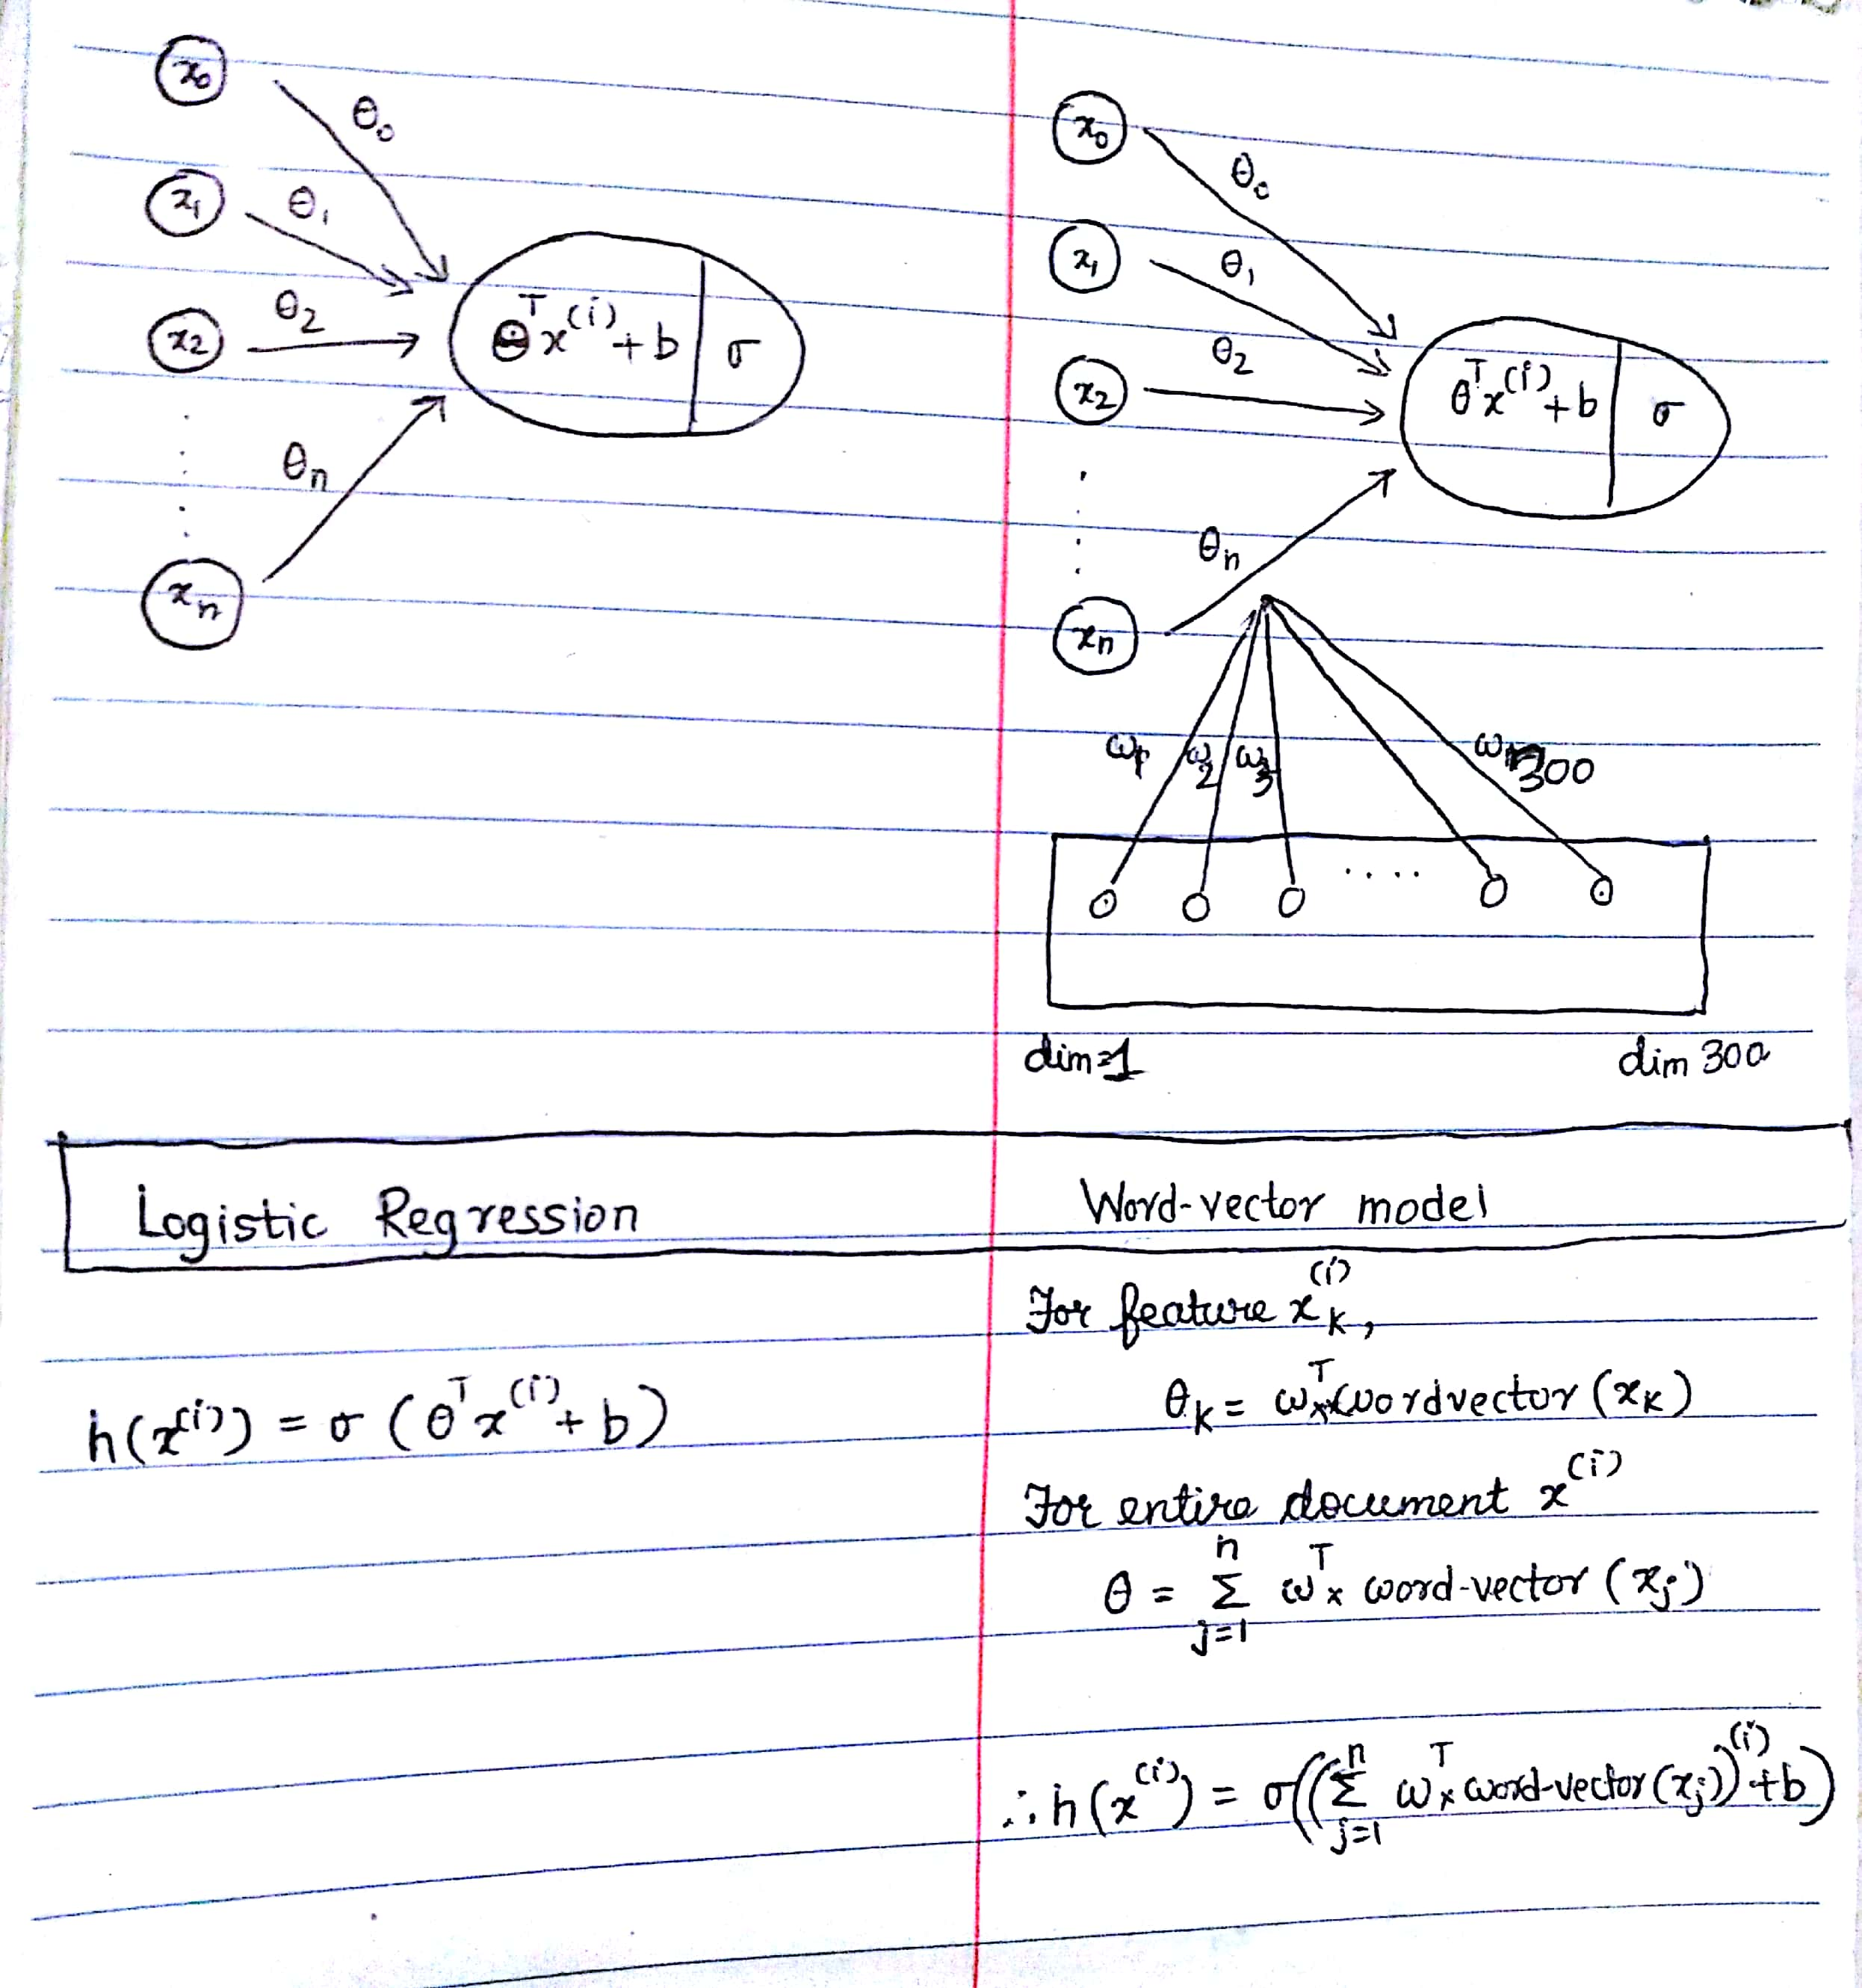
\includegraphics[width=16cm, height=10cm]{wordvec.jpg}\\[1cm]
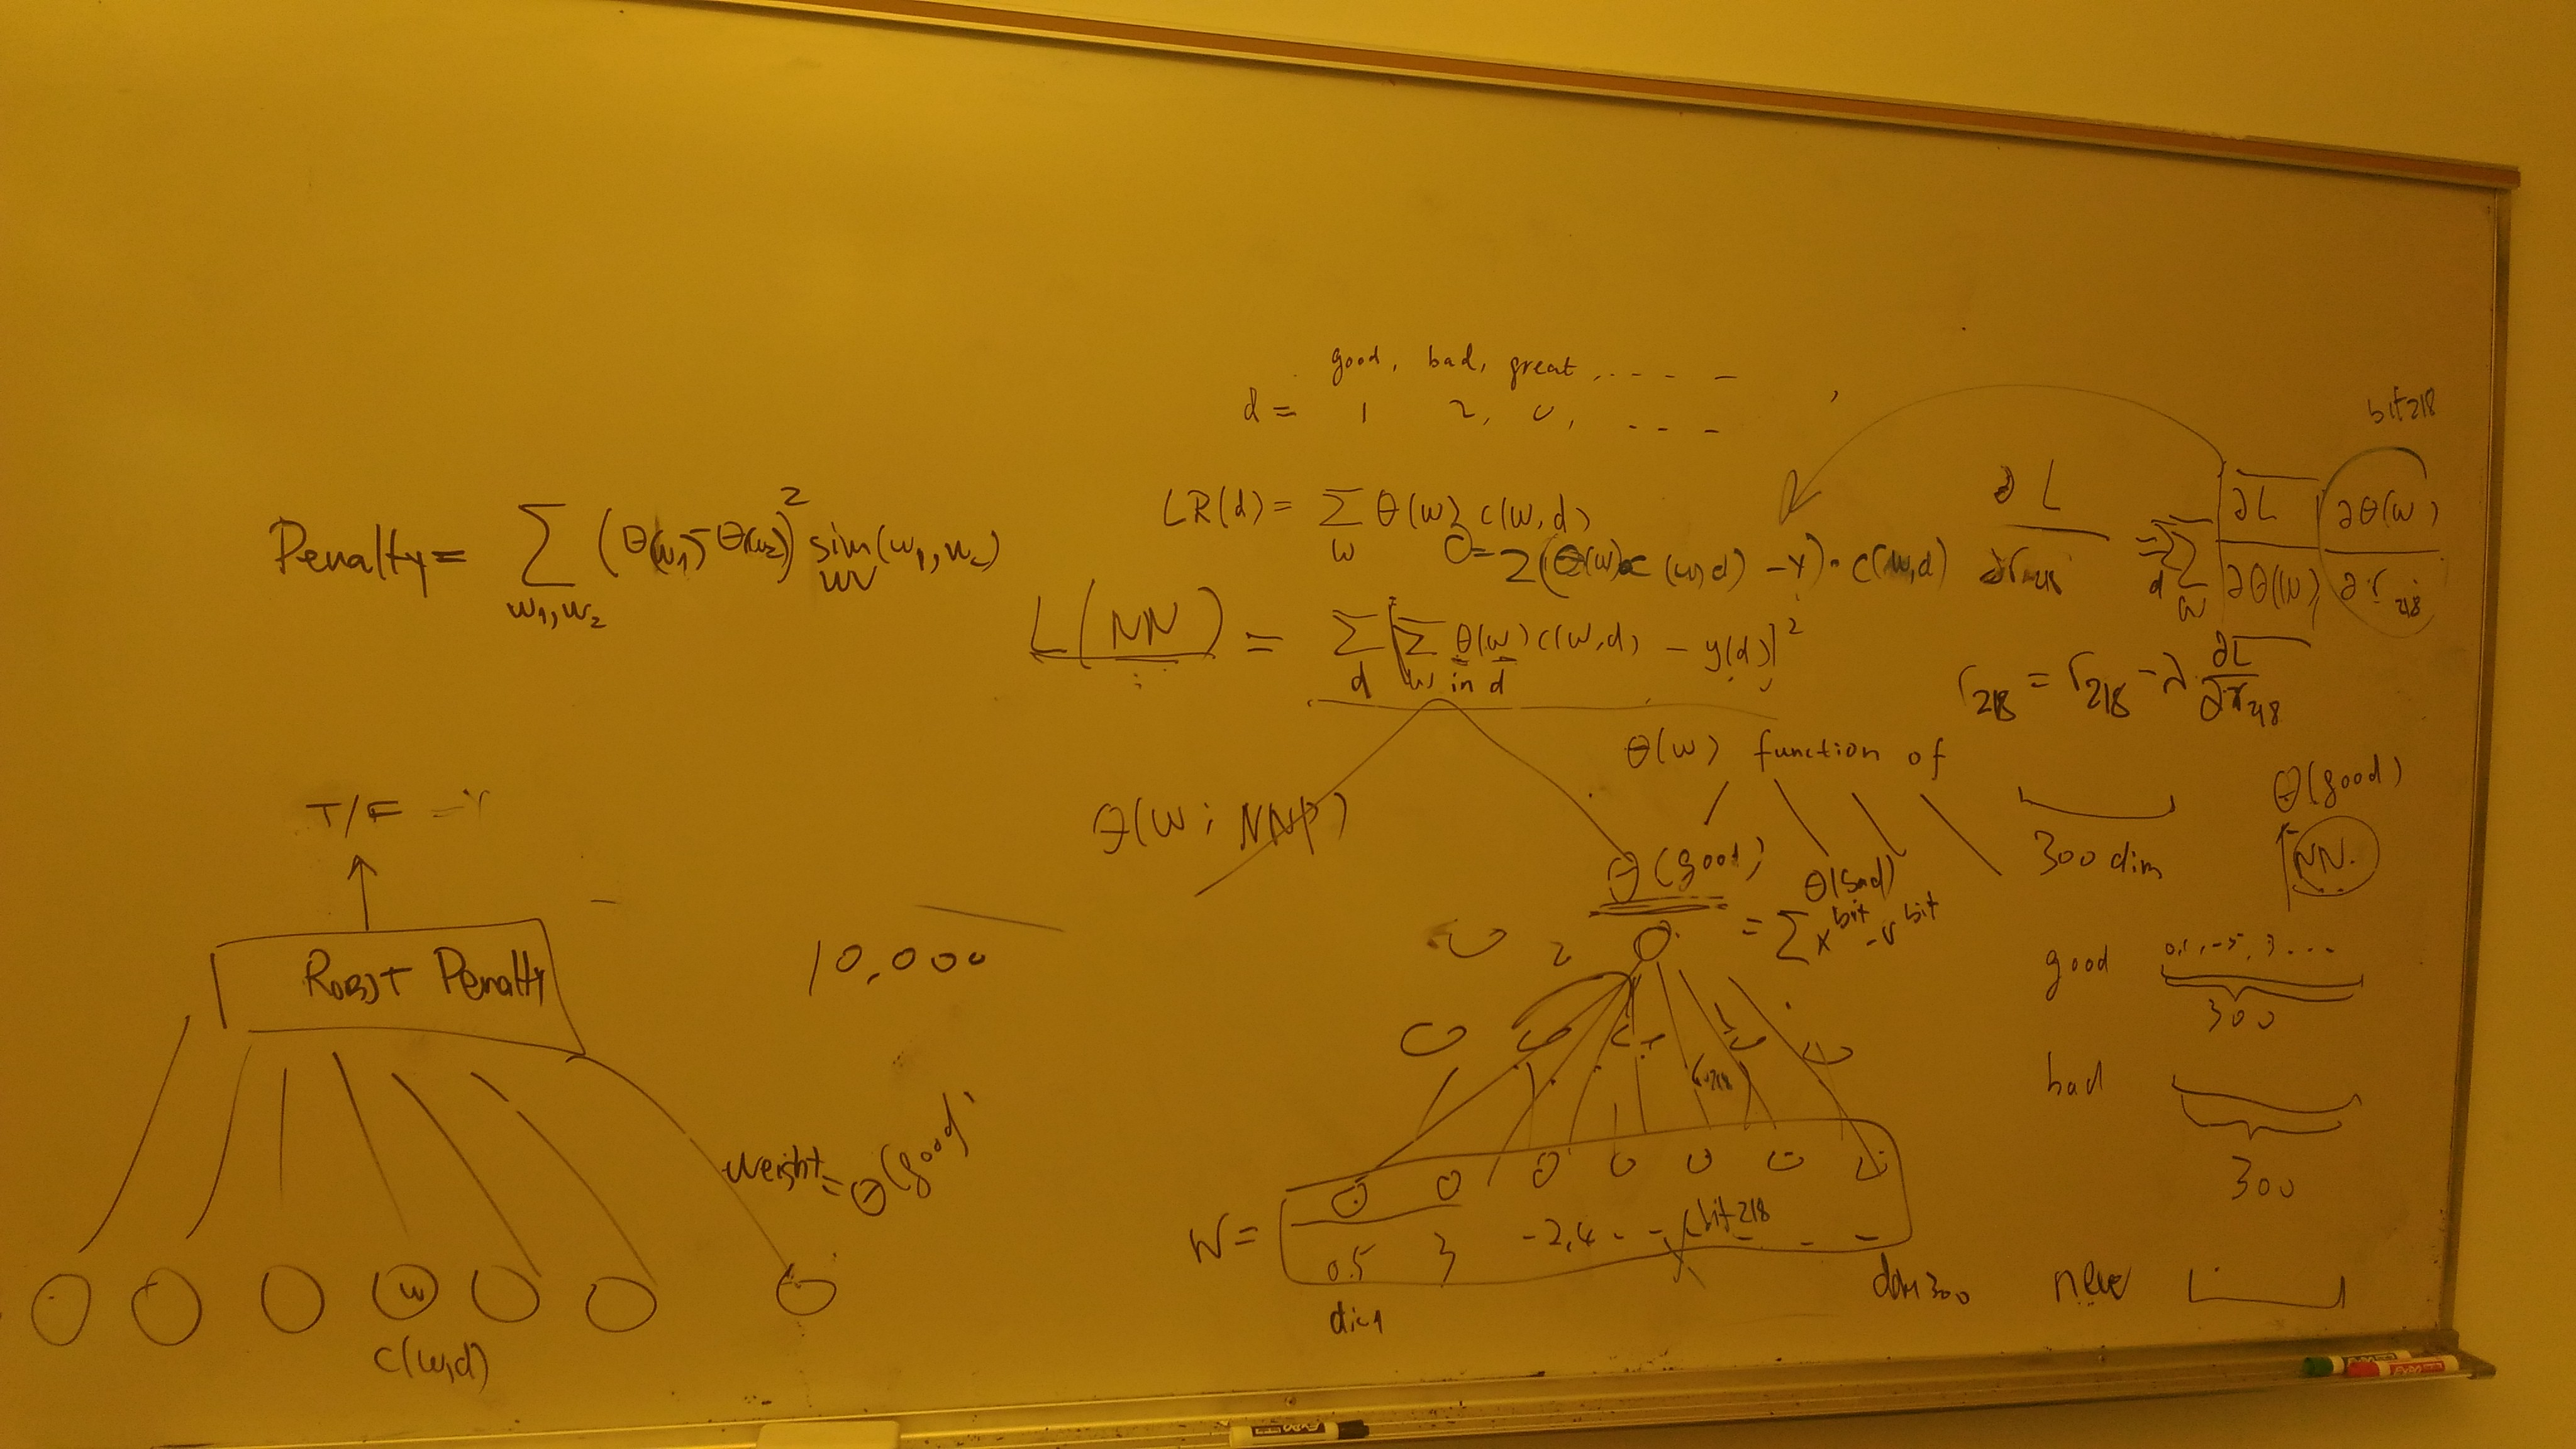
\includegraphics[width=16cm, height=10cm]{cheng.jpg}\\[1cm]

\chapter{Experiments}

Compare model performance with logistic regression on different datasets

\chapter{Applications}

\begin{itemize}
\item Explain why it could be useful on medical datasets which have specialized technical vocabulary

\item Other scenarios where this would be useful
\end{itemize}

\chapter{References}

\end{document}